
% 01-prologue/slides.tex, v. 1 (21/12/12)
% companion files to "Language and Computers"
% Dickinson, Brew, & Meurers (2013)

\documentclass{beamer}

% \usepackage{../styles/lgcomp}
\usepackage{graphicx}
\usepackage{forest,adjustbox}
\useforestlibrary{linguistics}
\forestapplylibrarydefaults{linguistics}
\usepackage{mrs}
\usepackage{avm}

\title{Introduction to NLP}
%\author[Sidebar Name]{First slide name}
\author{Alexandre Rademaker\thanks{Olga Zamaraeva}}
\institute{FGV/EMAp}

\subtitle{Parsing algorithms}
\date{May 9, 2018}
%\date{Your semester/date here}

\begin{document}
   
\begin{frame}
  \maketitle
\end{frame}

\section{Syntactic Parsing}

\begin{frame}
\frametitle{Overview}
\begin{itemize}
\item We will focus on the concept of parsing
\item and why naive parsing is inefficient
\item Dynamic programming idea
\item Then will briefly cover CKY
\item and then an assignment will ask you to study it in detail
\item we discussed probabilistic parsing
\end{itemize}
\end{frame}

\begin{frame}
\frametitle{Parsing}
\begin{itemize}
\item Recognizing string as input and assigning structure to it
\item Syntactic parsing: assigning syntactic structure
\item Semantic parsing: assigning semantic structure
\end{itemize}
\end{frame}

\begin{frame}
\frametitle{Syntactic Parsing}

Parsing: Making explicit structure that is inherent (implicit) in natural language strings
\begin{itemize}
\item What is that structure?
\item Why would we need it?
\end{itemize}
\end{frame}

\section{Parsing algorithms}

\begin{frame}[fragile]
\frametitle{Bottom Up vs. Top Down parsing}

\begin{verbatim}
         S
        /|\
        
        ???
        
   |  |  |  |  |  |
   a  b  c  d  d  f 
\end{verbatim}


\end{frame}

\begin{frame}
\frametitle{Recursive Top-Down Parsing}
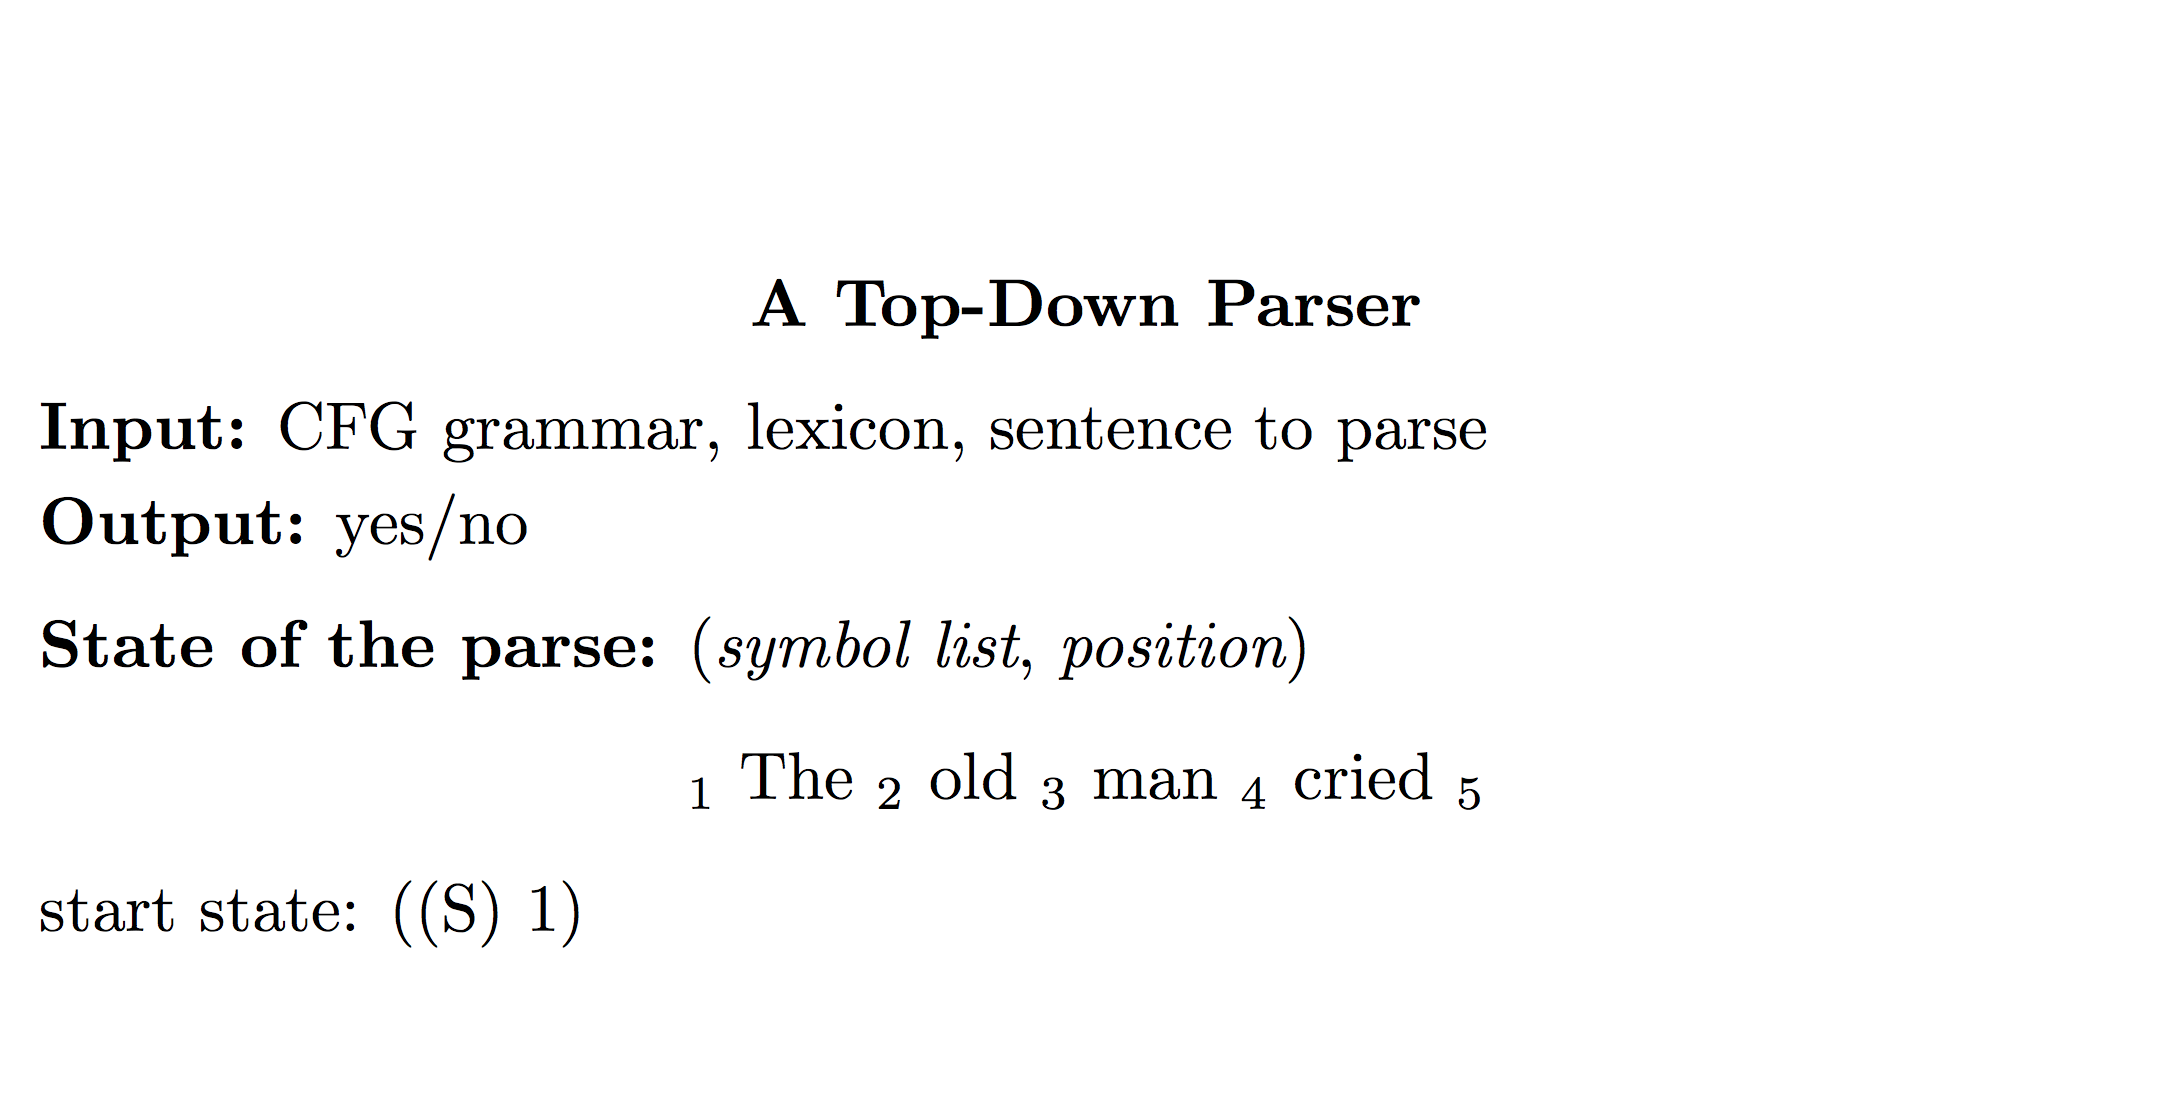
\includegraphics[width=\textwidth]{figures/top1}

{\tiny slide from: \url{https://www.cs.cornell.edu/courses/cs4740/2012sp/lectures/parsing-intro-4pp.pdf}}
\end{frame}

\begin{frame}
\frametitle{Recursive Top-Down Parsing}
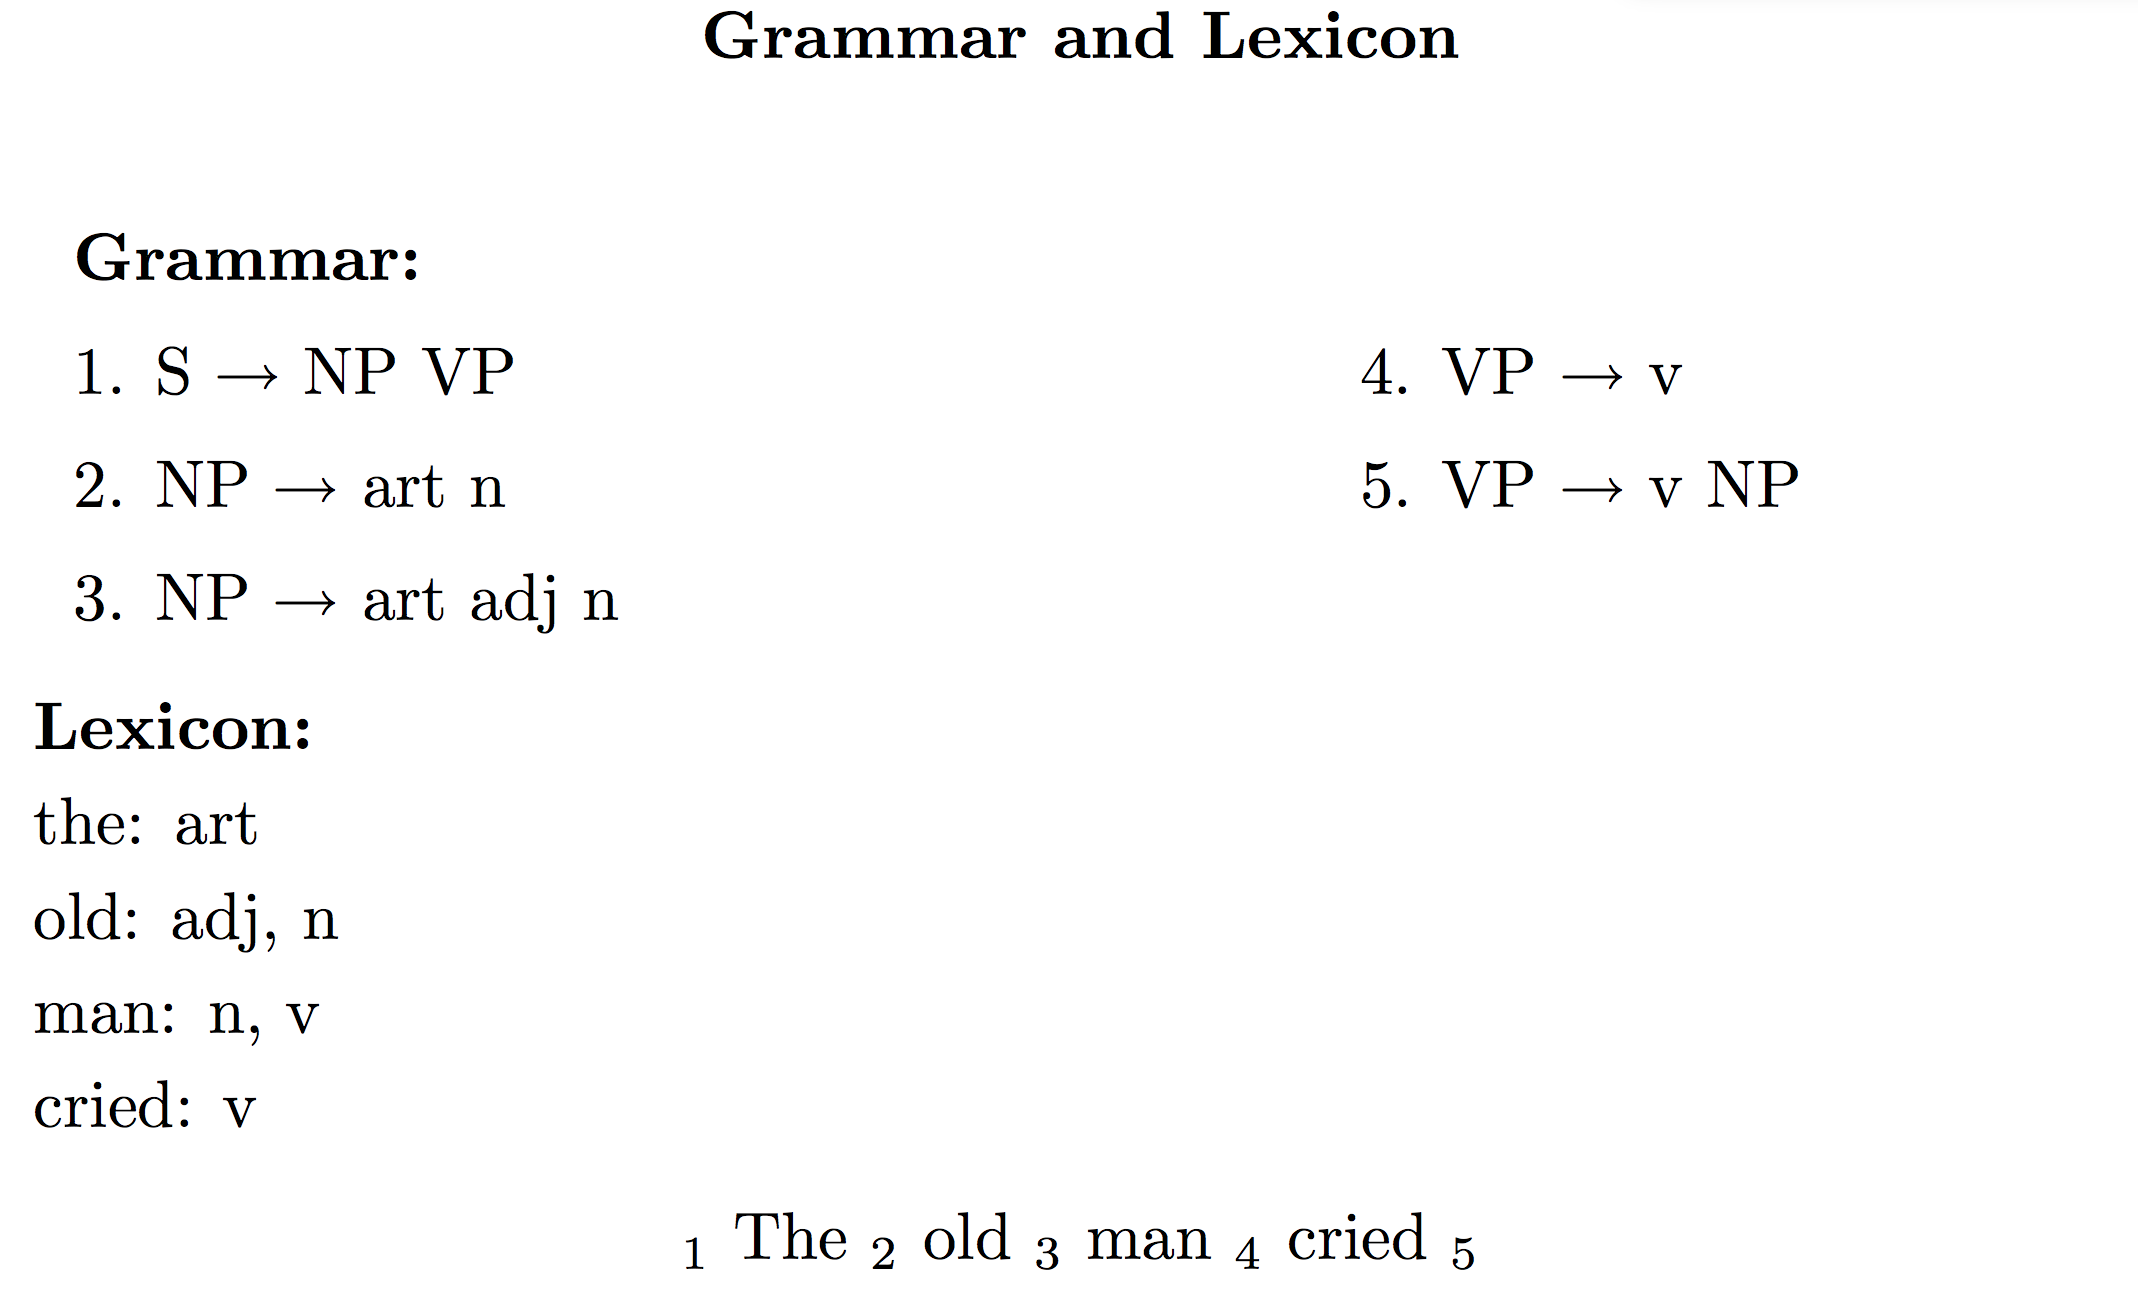
\includegraphics[width=\textwidth]{figures/top2}

{\tiny slide from: \url{https://www.cs.cornell.edu/courses/cs4740/2012sp/lectures/parsing-intro-4pp.pdf}}

\end{frame}


\begin{frame}
\frametitle{Recursive Top-Down Parsing}
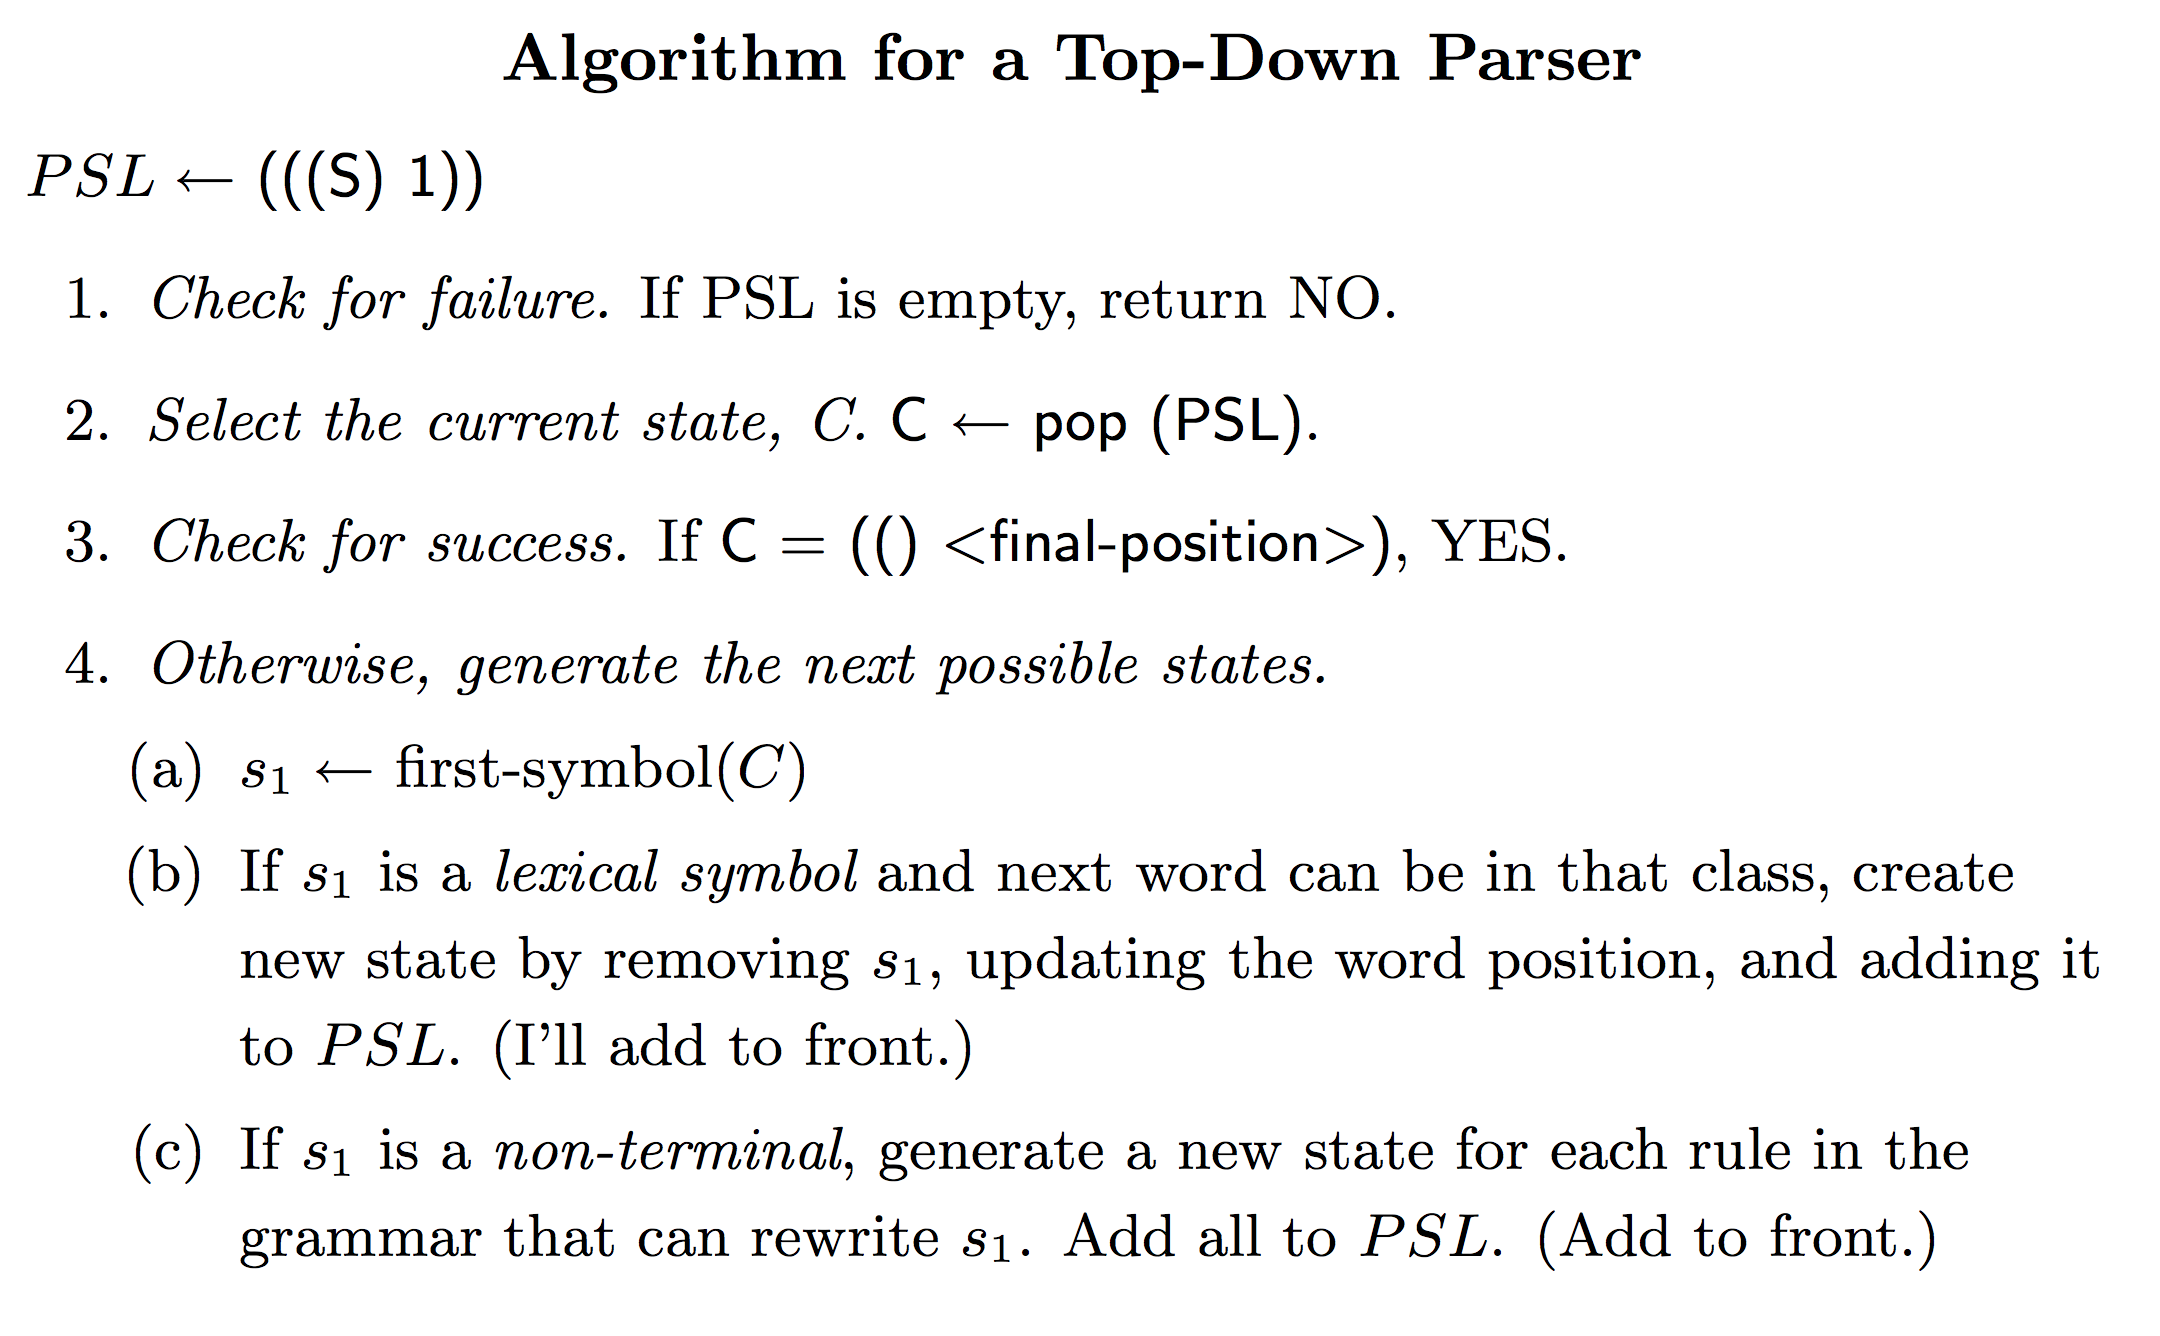
\includegraphics[width=\textwidth]{figures/top3}

{\tiny slide from: \url{https://www.cs.cornell.edu/courses/cs4740/2012sp/lectures/parsing-intro-4pp.pdf}}

\end{frame}

\begin{frame}
\frametitle{Recursive Top-Down Parsing}
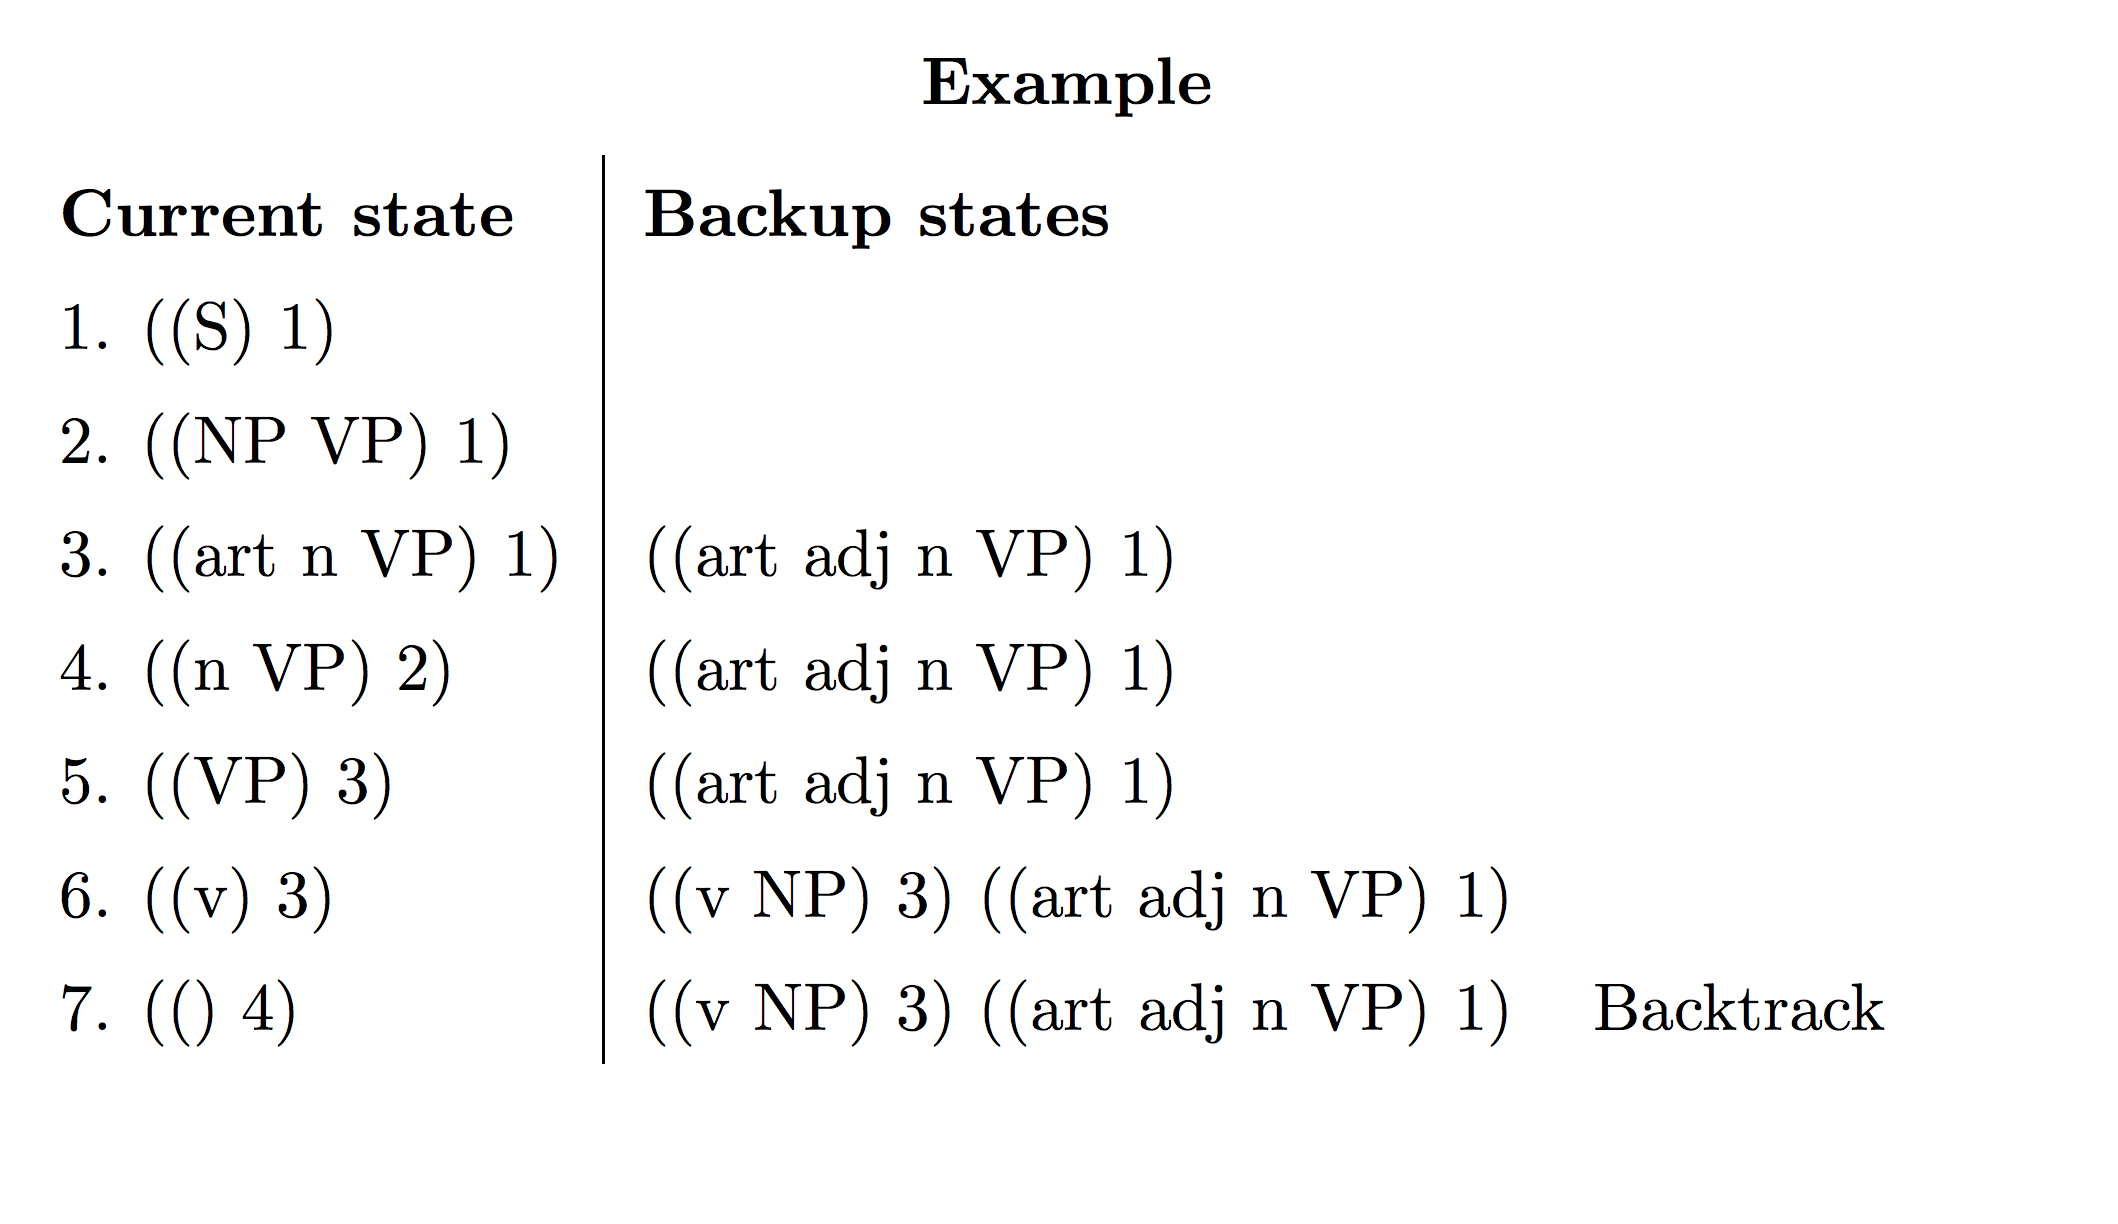
\includegraphics[width=\textwidth]{figures/top4}

{\tiny slide from: \url{https://www.cs.cornell.edu/courses/cs4740/2012sp/lectures/parsing-intro-4pp.pdf}}

\end{frame}


\begin{frame}
\frametitle{Recursive Top-Down Parsing}
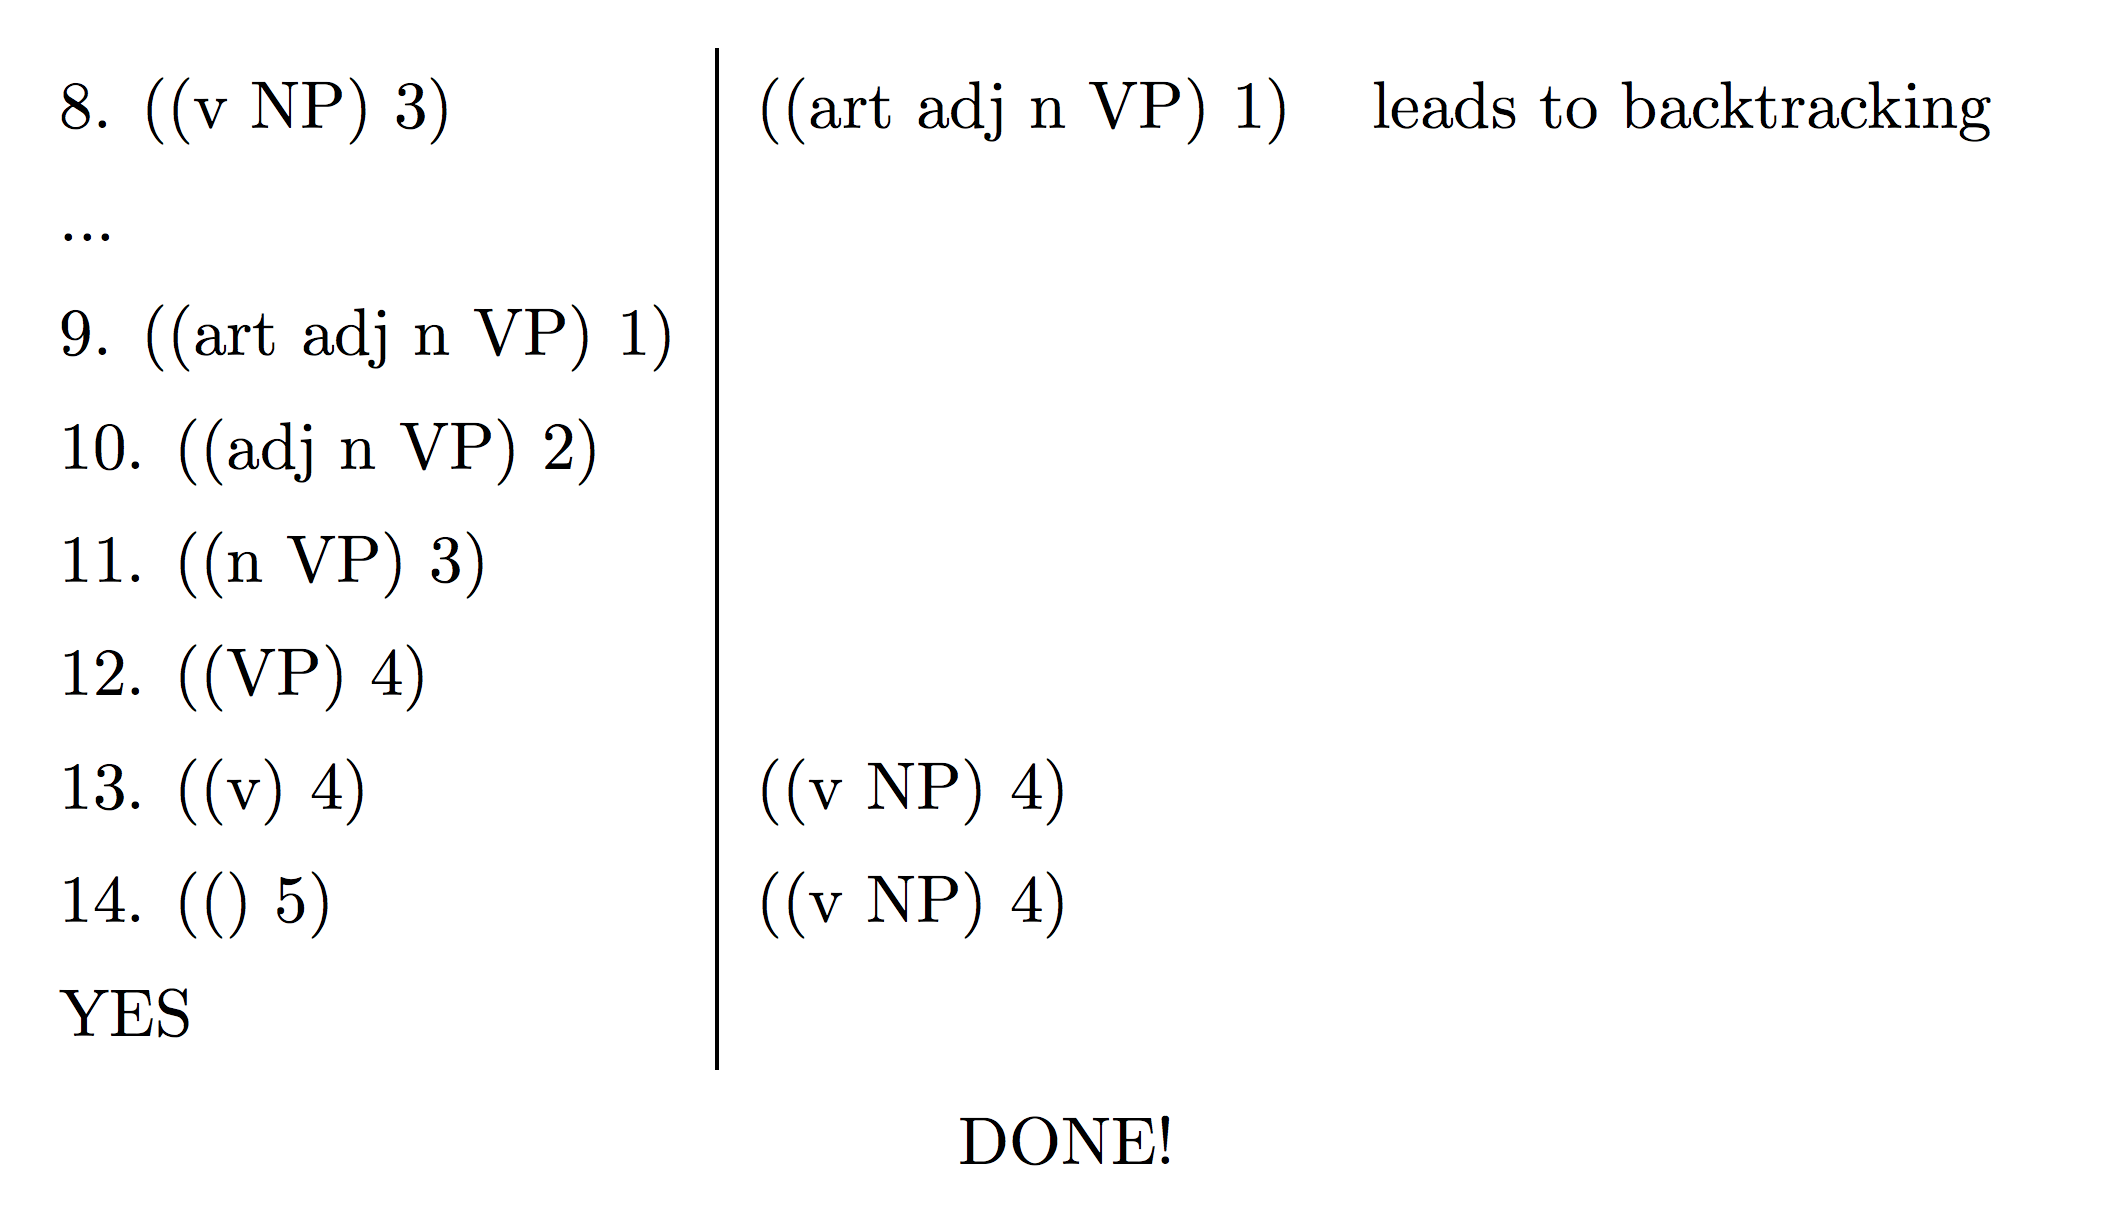
\includegraphics[width=\textwidth]{figures/top5}

{\tiny slide from: \url{https://www.cs.cornell.edu/courses/cs4740/2012sp/lectures/parsing-intro-4pp.pdf}}

\end{frame}

\begin{frame}
\frametitle{Recursive Top-Down Parsing}

\begin{itemize}
\item What is the time complexity of what we just saw?
\end{itemize}
\end{frame}

%\begin{frame}
%\frametitle{Recursive Parsing Running Time}
%
%S $\rightarrow$ A 
%
%A $\rightarrow$ a A b $\vert$ a A c $\vert$ $\epsilon$
%
%\begin{itemize}
%\item Consider a string $a^nc^n$
%\end{itemize}
%
%\end{frame}
%
%\begin{frame}
%\frametitle{Recursive Parsing Running Time}
%
%S $\rightarrow$ A 
%
%A $\rightarrow$ a A b $\vert$ a A c $\vert$ $\epsilon$
%
%\begin{itemize}
%\item Consider a string $a^nc^n$
%\item e.g. $_1a_2a_3a_4a_5c_6c_7c_8c_9$
%\end{itemize}
%
%\begin{tabular}{l|l|l}
%current state& backup states & input\\
%\hline
%((S) 1) && $a_2a_3a_4a_5c_6c_7c_8c_9$\\
%((A) 1) & &$a_2a_3a_4a_5c_6c_7c_8c_9$\\
%((Ab) 2) & ((Ac) 2) &$a_3a_4a_5c_6c_7c_8c_9$\\
%((Ab) 3) & ((Ac) 2) ((Ac) 3) &$a_4a_5c_6c_7c_8c_9$\\
%((Ab) 4) & ((Ac) 2) ((Ac) 3) ((Ac) 4) &$a_5c_6c_7c_8c_9$\\
%((Ab) 5) & ((Ac) 2) ((Ac) 3) ((Ac) 4) ((Ac) 5)&$c_6c_7c_8c_9$\\
%backtrack! & ((Ac) 2) ((Ac) 3) ((Ac) 4) ((Ac) 5)&$c_6c_7c_8c_9$\\
% ((Ac) 2)  &((Ac) 3) ((Ac) 4) ((Ac) 5)&$a_3a_4a_5c_6c_7c_8c_9$\\
%\end{tabular}
%
%\end{frame}
%
%\begin{frame}
%\frametitle{Recursive Parsing Running Time}
%
%S $\rightarrow$ A 
%
%A $\rightarrow$ a A b $\vert$ a A c $\vert$ $\epsilon$
%
%\begin{itemize}
%\item Consider a string $a^nc^n$
%\item e.g. $_1a_2a_3a_4a_5c_6c_7c_8c_9$
%\end{itemize}
%
%\begin{footnotesize}
%\begin{tabular}{l|l|l}
%current state& backup states & input\\
%\hline
% ((Ac) 2)  &((Ac) 3) ((Ac) 4) ((Ac) 5)&$a_3a_4a_5c_6c_7c_8c_9$\\
% ((Abc) 3)  &((Acc) 3) ((Ac) 3) ((Ac) 4) ((Ac) 5)&$a_4a_5c_6c_7c_8c_9$\\
% ((Abc) 4)  &((Acc) 4) ((Acc) 3) ((Ac) 3) ((Ac) 4) ((Ac) 5)&$a_5c_6c_7c_8c_9$\\
% ((Abc) 5)  &((Acc) 5) ((Acc) 4) ((Acc) 3) ((Ac) 3) ((Ac) 4) ((Ac) 5)&$c_6c_7c_8c_9$\\
% backtrack!  &((Acc) 5)((Acc) 4)  ((Acc) 3) ((Ac) 3) ((Ac) 4) ((Ac) 5)&$c_6c_7c_8c_9$\\
% ((Acc) 5)  &((Acc) 4) ((Acc) 3) ((Ac) 3) ((Ac) 4) ((Ac) 5)&$c_6c_7c_8c_9$\\
% backtrack!  &((Acc) 5) ((Acc) 4) ((Acc) 3) ((Ac) 3) ((Ac) 4) ((Ac) 5)&$c_6c_7c_8c_9$\\
% ((Acc) 4)  &((Acc) 3) ((Ac) 3) ((Ac) 4) ((Ac) 5)&$a_5c_6c_7c_8c_9$\\
%\end{tabular}
%\end{footnotesize}
%\end{frame}
%
%\begin{frame}
%\frametitle{Recursive Parsing Running Time}
%
%S $\rightarrow$ A 
%
%A $\rightarrow$ a A b $\vert$ a A c $\vert$ $\epsilon$
%
%\begin{itemize}
%\item Consider a string $a^nc^n$
%\item e.g. $_1a_2a_3a_4a_5c_6c_7c_8c_9$
%\end{itemize}
%
%\begin{footnotesize}
%\begin{tabular}{l|l|l}
%current state& backup states & input\\
%\hline
% ((Acc) 4)  &((Acc) 3) ((Ac) 3) ((Ac) 4) ((Ac) 5)&$a_5c_6c_7c_8c_9$\\
% ((Abcc) 5)  &((Accc) 5) ((Acc) 3) ((Ac) 3) ((Ac) 4) ((Ac) 5)&$c_6c_7c_8c_9$\\
% backtrack! &((Accc) 5) ((Acc) 3) ((Ac) 3) ((Ac) 4) ((Ac) 5)&$c_6c_7c_8c_9$\\
% ((Accc) 5)  & ((Acc) 3) ((Ac) 3) ((Ac) 4) ((Ac) 5)&$c_6c_7c_8c_9$\\
% ((Abccc) 6)  & ((Acccc) 6) ((Acc) 3) ((Ac) 3) ((Ac) 4) ((Ac) 5)&$c_7c_8c_9$\\
% backtrack!  & ((Acccc) 6) ((Acc) 3) ((Ac) 3) ((Ac) 4) ((Ac) 5)&$c_7c_8c_9$\\
% ((Acccc) 6)  & ((Acc) 3) ((Ac) 3) ((Ac) 4) ((Ac) 5)&$c_7c_8c_9$\\
%\end{tabular}
%\end{footnotesize}
%
%\end{frame}


\begin{frame}
\frametitle{Recursive Top-Down Parsing}

\begin{itemize}
\item What is the time complexity of what we just saw?
\begin{itemize}
\item {\bf Exponential} in n!
\item (Meaning, as we increase the length of input, the time to do parsing increases {\bf exponentially})
\item (Which is very very bad)
\end{itemize}
\end{itemize}
\end{frame}

\begin{frame}
\frametitle{**Optional exercise: Recursive Parsing Running Time}

S $\rightarrow$ A 

A $\rightarrow$ a A b $\vert$ a A c $\vert$ $\epsilon$

\begin{itemize}
\item Consider a string $a^nc^n$
\item Convince yourself that you will expand A $2^n$ times
\end{itemize}

\end{frame}


%\begin{frame}
%\frametitle{Top-Down Parsing}
%
%{\it Book the flight through Houston }
%
%\begin{itemize}
%\item {\it Book the flight through Houston } must match S
%\item Therefore it must match {\bf NP VP} or Aux {\bf NP VP} or {\bf VP}
%\item Viable options are {\bf NP VP} and {\bf VP} (why?)
%\item Explore {\bf NP VP} (put {\bf VP} on the stack):
%\begin{itemize}
%\item {\it book} can be NP; but no way to match the rest of the string
%\item Therefore backtrack 
%\end{itemize}
%\item ...and explore {\bf VP}:
%\begin{itemize}
%\item Must match \{Verb, Verb NP, Verb NP PP, Verb PP, VP PP\}
%\item Viable options: {\bf Verb NP PP} and {\bf Verb NP}
%\item (Cut to the chase: we can expand both successfully)
%\end{itemize}
%\end{itemize}
%\end{frame}


\begin{frame}
\frametitle{Example}
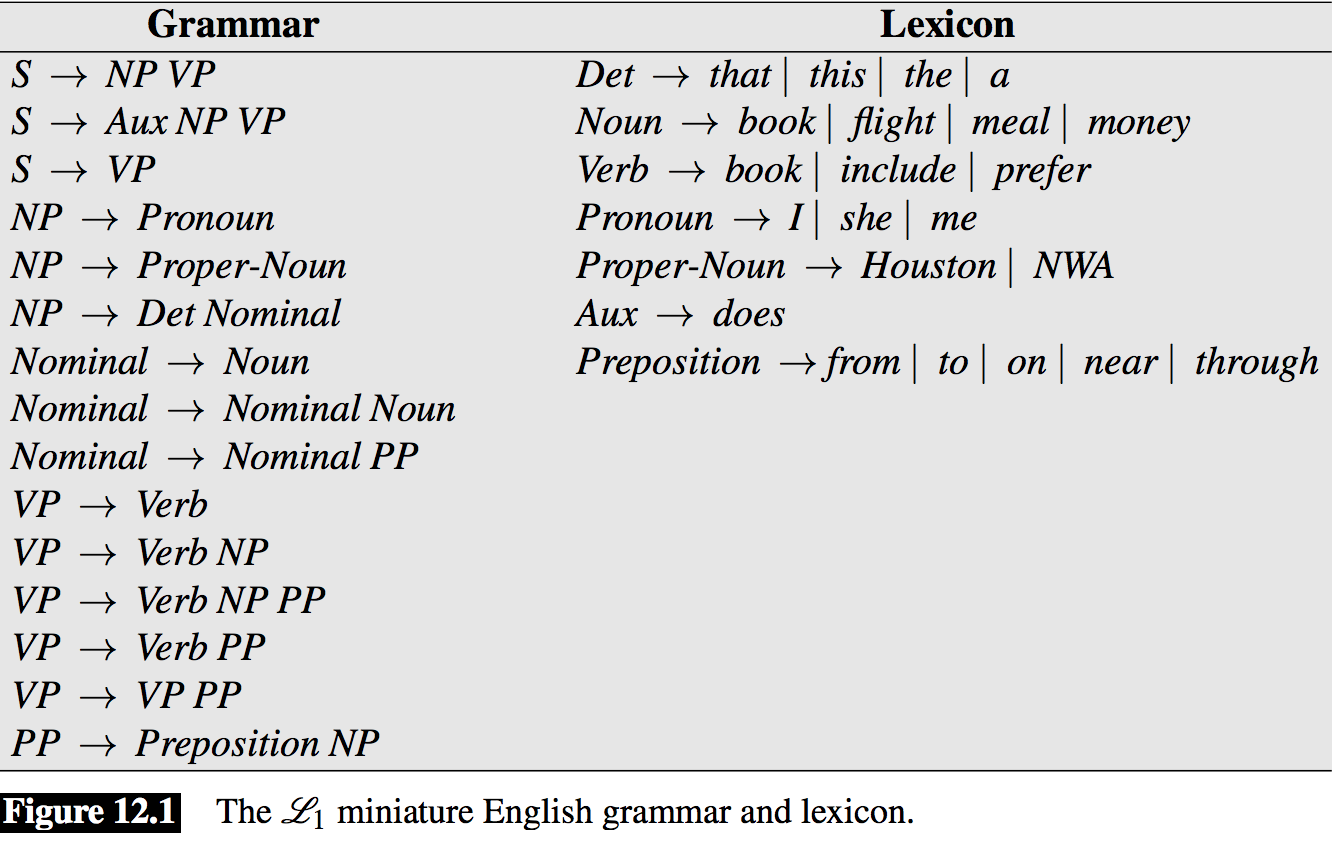
\includegraphics[width=\textwidth]{figures/grammar}
\end{frame}

%\begin{frame}
%\frametitle{Bottom-Up Parsing}
%
%{\it Book the flight through Houston }
%
%\small
%\begin{itemize}
%\item Can I rewrite {\it book}?
%\begin{itemize}
%\item Noun, Nominal, Verb, VP, S
%\item S is the Start symbol but we haven't used all input
%\item Can I rewrite \{Noun, Nominal, Verb, VP, S\} {\it the}?
%\item Rewrite {\it the} as Det
%\item Can I rewrite \{Noun, Nominal, Verb, VP, S\} Det?
%\item Can I rewrite \{Noun, Nominal, Verb, VP, S\} Det {\it flight}?
%\item \{Noun, Nominal, Verb, VP, S\} Det Nominal
%\item rewrite Det Nominal as NP
%\item Can I rewrite \{Noun, Nominal, Verb, VP, S\} NP?
%\item rewrite Verb NP as VP
%\item Can I rewrite VP {\it through}?
%\item Can I rewrite VP P?
%\item Can I rewrite VP P {\it Houston}?
%\item Can I rewrite VP P Proper-Noun?
%\item Can I rewrite VP PP?
%\item VP $\rightarrow$ VP PP
%\item S $\rightarrow$ VP {\bf (Done!)}
%\end{itemize}
%\end{itemize}
%\end{frame}


\begin{frame}
\frametitle{Bottom-up parsing}
Book the flight through Houston
\end{frame}

\begin{frame}
\frametitle{Bottom-up parsing}
\begin{forest}
[N[Book]]
\end{forest}
\begin{forest}
[D[the]]
\end{forest}
\begin{forest}
[N[flight]]
\end{forest}
\begin{forest}
[P[through]]
\end{forest}
\begin{forest}
[PN[Houston]]
\end{forest}
\end{frame}

\begin{frame}
\frametitle{Bottom-up parsing}
\begin{forest}
[Nom[N[Book]]]
\end{forest}
\begin{forest}
[D[the]]
\end{forest}
\begin{forest}
[Nom[N[flight]]]
\end{forest}
\begin{forest}
[P[through]]
\end{forest}
\begin{forest}
[PN[Houston]]
\end{forest}
\end{frame}

\begin{frame}
\frametitle{Bottom-up parsing}
\begin{forest}
[Nom[N[Book]]]
\end{forest}
\begin{forest}
[NP
[D[the]]
[Nom[N[flight]]]]
\end{forest}
\begin{forest}
[PP
[P[through]]
[PN[Houston]]]
\end{forest}

No more possibilities! Backtrack...
\end{frame}

\begin{frame}
\frametitle{Bottom-up parsing}
\begin{forest}
[Nom[N[Book]]]
\end{forest}
\begin{forest}
[D[the]]
\end{forest}
\begin{forest}
[Nom[N[flight]]]
\end{forest}
\begin{forest}
[PP
[P[through]]
[PN[Houston]]]
\end{forest}
\end{frame}

\begin{frame}
\frametitle{Bottom-up parsing}
\begin{forest}
[Nom[N[Book]]]
\end{forest}
\begin{forest}
[D[the]]
\end{forest}
\begin{forest}
[Nom
[Nom[N[flight]]]
[PP
[P[through]]
[PN[Houston]]]]
\end{forest}
\end{frame}

\begin{frame}
\frametitle{Bottom-up parsing}
\begin{forest}
[Nom[N[Book]]]
\end{forest}
\begin{forest}
[NP
[D[the]]
[Nom
[Nom[N[flight]]]
[PP
[P[through]]
[PN[Houston]]]]]
\end{forest}

No more possibilities! Backtrack... Up to where?..
\end{frame}

\begin{frame}
\frametitle{Bottom-up parsing}
Backtrack to the very beginning, actually!

\vspace{2cm}

Book the flight through Houston
\end{frame}

\begin{frame}
\frametitle{Bottom-up parsing}
\begin{forest}
[V[Book]]
\end{forest}
\begin{forest}
[D[the]]
\end{forest}
\begin{forest}
[N[flight]]
\end{forest}
\begin{forest}
[P[through]]
\end{forest}
\begin{forest}
[PN[Houston]]
\end{forest}
\end{frame}

\begin{frame}
\frametitle{Bottom-up parsing}
\begin{forest}
[V[Book]]
\end{forest}
\begin{forest}
[D[the]]
\end{forest}
\begin{forest}
[Nom[N[flight]]]
\end{forest}
\begin{forest}
[P[through]]
\end{forest}
\begin{forest}
[PN[Houston]]
\end{forest}
\end{frame}

\begin{frame}
\frametitle{Bottom-up parsing}
\begin{forest}
[V[Book]]
\end{forest}
\begin{forest}
[NP
[D[the]]
[Nom[N[flight]]]]
\end{forest}
\begin{forest}
[PP
[P[through]]
[PN[Houston]]]
\end{forest}
\end{frame}

\begin{frame}
\frametitle{Bottom-up parsing}
\begin{forest}
[VP
[V[Book]]
[NP
[D[the]]
[Nom[N[flight]]]]]
\end{forest}
\begin{forest}
[PP
[P[through]]
[PN[Houston]]]
\end{forest}
\end{frame}

\begin{frame}
\frametitle{Bottom-up parsing}
\begin{forest}
[VP
[VP
[V[Book]]
[NP
[D[the]]
[Nom[N[flight]]]]]
[PP
[P[through]]
[PN[Houston]]]]
\end{forest}
\end{frame}

\begin{frame}
\frametitle{Bottom-up parsing}
\begin{forest}
[S
[VP
[VP
[V[Book]]
[NP
[D[the]]
[Nom[N[flight]]]]]
[PP
[P[through]]
[PN[Houston]]]]]
\end{forest}
\end{frame}

\begin{frame}
\frametitle{Bottom-up parsing}
Or, we could have instead done:

\begin{forest}
[V[Book]]
\end{forest}
\begin{forest}
[D[the]]
\end{forest}
\begin{forest}
[Nom[N[flight]]]
\end{forest}
\begin{forest}
[PP
[P[through]]
[PN[Houston]]]
\end{forest}
\end{frame}

\begin{frame}
\frametitle{Bottom-up parsing}
\begin{forest}
[V[Book]]
\end{forest}
\begin{forest}
[D[the]]
\end{forest}
\begin{forest}
[Nom
[Nom[N[flight]]]
[PP
[P[through]]
[PN[Houston]]]]
\end{forest}
\end{frame}

\begin{frame}
\frametitle{Bottom-up parsing}
\begin{forest}
[V[Book]]
\end{forest}
\begin{forest}
[NP
[D[the]]
[Nom
[Nom[N[flight]]]
[PP
[P[through]]
[PN[Houston]]]]]
\end{forest}
\end{frame}

\begin{frame}
\frametitle{Bottom-up parsing}
\begin{forest}
[VP
[V[Book]]
[NP
[D[the]]
[Nom
[Nom[N[flight]]]
[PP
[P[through]]
[PN[Houston]]]]]]
\end{forest}
\end{frame}

\begin{frame}
\frametitle{Bottom-up parsing}
\begin{forest}
[S
[VP
[V[Book]]
[NP
[D[the]]
[Nom
[Nom[N[flight]]]
[PP
[P[through]]
[PN[Houston]]]]]]]
\end{forest}
\end{frame}

\begin{frame}
\frametitle{How do we make sure we get both trees?}

\begin{itemize}
\item Go through {\bf all} possibilities for productions
\end{itemize}
\end{frame}


\begin{frame}
\frametitle{Top-Down Parsing}
\begin{center}
\begin{forest}
[S[]]
\end{forest}
\end{center}
\end{frame}


\begin{frame}
\frametitle{Top-Down Parsing}
\begin{center}
\begin{forest}
[S[NP][VP]]
\end{forest}
\end{center}
\end{frame}

\begin{frame}
\frametitle{Top-Down Parsing}
\begin{center}
\begin{forest}
[S[NP[Pronoun]][VP]]
\end{forest}
\end{center}
\end{frame}

\begin{frame}
\frametitle{Top-Down Parsing}
\begin{center}
\begin{forest}
[S[NP][VP]]
\end{forest}
\end{center}
\end{frame}

\begin{frame}
\frametitle{Top-Down Parsing}
\begin{center}
\begin{forest}
[S[NP[PN]][VP]]
\end{forest}
\end{center}
\end{frame}

\begin{frame}
\frametitle{Top-Down Parsing}
\begin{center}
\begin{forest}
[S[NP][VP]]
\end{forest}
\end{center}
\end{frame}

\begin{frame}
\frametitle{Top-Down Parsing}
\begin{center}
\begin{forest}
[S[NP[D][Nom]][VP]]
\end{forest}
\end{center}
\end{frame}

\begin{frame}
\frametitle{Top-Down Parsing}
\begin{center}
\begin{forest}
[S[NP][VP]]
\end{forest}
\end{center}
\end{frame}

\begin{frame}
\frametitle{Top-Down Parsing}
\begin{center}
\begin{forest}
[S[]]
\end{forest}
\end{center}
\end{frame}

\begin{frame}
\frametitle{Top-Down Parsing}
\begin{center}
\begin{forest}
[S[Aux][NP][VP]]
\end{forest}
\end{center}
\end{frame}

\begin{frame}
\frametitle{Top-Down Parsing}
\begin{center}
\begin{forest}
[S[]]
\end{forest}
\end{center}
\end{frame}

\begin{frame}
\frametitle{Top-Down Parsing}
\begin{center}
\begin{forest}
[S[VP]]
\end{forest}
\end{center}
\end{frame}

\begin{frame}
\frametitle{Top-Down Parsing}
\begin{center}
\begin{forest}
[S[VP[V]]]
\end{forest}
\end{center}
\end{frame}

\begin{frame}
\frametitle{Top-Down Parsing}
\begin{center}
\begin{forest}
[S[VP[V[Book]]]]
\end{forest}
\end{center}

Yes, but we have more input still...
\end{frame}

\begin{frame}
\frametitle{Top-Down Parsing}
\begin{center}
\begin{forest}
[S[VP [V] [NP]]]
\end{forest}
\end{center}
\end{frame}

\begin{frame}
\frametitle{Top-Down Parsing}
\begin{center}
\begin{forest}
[S[VP [V[Book]] [NP]]]
\end{forest}
\end{center}
\end{frame}

\begin{frame}
\frametitle{Top-Down Parsing}
\begin{center}
\begin{forest}
[S[VP [V[Book]] [NP[Pronoun]]]]
\end{forest}
\end{center}
\end{frame}

\begin{frame}
\frametitle{Top-Down Parsing}
\begin{center}
\begin{forest}
[S[VP [V[Book]] [NP]]]
\end{forest}
\end{center}
\end{frame}

\begin{frame}
\frametitle{Top-Down Parsing}
\begin{center}
\begin{forest}
[S[VP [V[Book]] [NP[PN]]]]
\end{forest}
\end{center}
\end{frame}

\begin{frame}
\frametitle{Top-Down Parsing}
\begin{center}
\begin{forest}
[S[VP [V[Book]] [NP]]]
\end{forest}
\end{center}
\end{frame}

\begin{frame}
\frametitle{Top-Down Parsing}
\begin{center}
\begin{forest}
[S[VP [V[Book]] [NP[D][Nom]]]]
\end{forest}
\end{center}
\end{frame}

\begin{frame}
\frametitle{Top-Down Parsing}
\begin{center}
\begin{forest}
[S[VP [V[Book]] [NP[D [the]][Nom]]]]
\end{forest}
\end{center}
\end{frame}

\begin{frame}
\frametitle{Top-Down Parsing}
\begin{center}
\begin{forest}
[S[VP [V[Book]] [NP[D [the]][Nom [N]]]]]
\end{forest}
\end{center}
\end{frame}

\begin{frame}
\frametitle{Top-Down Parsing}
\begin{center}
\begin{forest}
[S[VP [V[Book]] [NP[D [the]][Nom [N[flight]]]]]]
\end{forest}
\end{center}

Yes, but we have more input still...
\end{frame}

\begin{frame}
\frametitle{Top-Down Parsing}
\begin{center}
\begin{forest}
[S[VP [V[Book]] [NP[D [the]][Nom [Nom][N]]]]]
\end{forest}
\end{center}
\end{frame}

\begin{frame}
\frametitle{Top-Down Parsing}
\begin{center}
\begin{forest}
[S[VP [V[Book]] [NP[D [the]][Nom [Nom[N]][N]]]]]
\end{forest}
\end{center}
\end{frame}


\begin{frame}
\frametitle{Top-Down Parsing}
\begin{small}
\begin{center}
\begin{forest}
[S[VP [V[Book]] [NP[D [the]][Nom [Nom[N [flight]]][N]]]]]
\end{forest}
\end{center}
\end{small}

Nope... Backtrack again...
\end{frame}

\begin{frame}
\frametitle{Top-Down Parsing}
\begin{center}
\begin{forest}
[S[VP [V[Book]] [NP[D [the]][Nom]]]]
\end{forest}
\end{center}
\end{frame}

\begin{frame}
\frametitle{Top-Down Parsing}
\begin{center}
\begin{forest}
[S[VP [V[Book]] [NP[D [the]][Nom[Nom][PP]]]]]
\end{forest}
\end{center}
\end{frame}

\begin{frame}
\frametitle{Top-Down Parsing}
\begin{center}
\begin{forest}
[S[VP [V[Book]] [NP[D [the]][Nom[Nom[N]][PP]]]]]
\end{forest}
\end{center}
\end{frame}

\begin{frame}
\frametitle{Top-Down Parsing}
\begin{center}
\begin{forest}
[S[VP [V[Book]] [NP[D [the]][Nom[Nom[N[flight]]][PP]]]]]
\end{forest}
\end{center}
\end{frame}

\begin{frame}
\frametitle{Top-Down Parsing}
\begin{center}
\begin{forest}
[S[VP [V[Book]] [NP[D [the]][Nom[Nom[N[flight]]][PP[P][NP]]]]]]
\end{forest}
\end{center}
\end{frame}

\begin{frame}
\frametitle{Top-Down Parsing}
\begin{center}
\begin{forest}
[S[VP [V[Book]] [NP[D [the]][Nom[Nom[N[flight]]][PP[P[through]][NP]]]]]]
\end{forest}
\end{center}
\end{frame}

\begin{frame}
\frametitle{Top-Down Parsing}
\begin{center}
\begin{forest}
[S[VP [V[Book]] [NP[D [the]][Nom[Nom[N[flight]]][PP[P[through]][NP[Pronoun]]]]]]]
\end{forest}
\end{center}
\end{frame}

\begin{frame}
\frametitle{Top-Down Parsing}
\begin{center}
\begin{forest}
[S[VP [V[Book]] [NP[D [the]][Nom[Nom[N[flight]]][PP[P[through]][NP]]]]]]
\end{forest}
\end{center}
\end{frame}

\begin{frame}
\frametitle{Top-Down Parsing}
\begin{center}
\begin{forest}
[S[VP [V[Book]] [NP[D [the]][Nom[Nom[N[flight]]][PP[P[through]][NP [PN]]]]]]]
\end{forest}
\end{center}
\end{frame}

\begin{frame}
\frametitle{Top-Down Parsing}
\begin{small}
\begin{center}
\begin{forest}
[S[VP [V[Book]] [NP[D [the]][Nom[Nom[N[flight]]][PP[P[through]][NP [PN [Houston]]]]]]]]
\end{forest}
\end{center}
\end{small}
\end{frame}

\begin{frame}
\frametitle{Top-Down Parsing}
\begin{itemize}
\item Could we have gotten the second tree by top-down parsing?
\end{itemize}
\end{frame}


\begin{frame}
\frametitle{Top-Down Parsing}
\begin{itemize}
\item Could we have gotten the second tree by top-down parsing?
\begin{itemize}
\item Yes; it is a matter of which rule happened to be on the top of the stack
\item We grabbed {\bf VP} $\rightarrow$ {\bf V NP}
\item But the option {\bf VP} $\rightarrow$ {\bf VP PP} is also on the stack somewhere
\item Thus the returned parse is subject to an arbitrary listing of rules in the grammar
\end{itemize}
\end{itemize}
\end{frame}

\begin{frame}[fragile]
\frametitle{Bottom Up vs. Top Down parsing}

%\begin{small}
\begin{itemize}
\item Top-down parsers do not waste time exploring hypotheses not leading to S
\begin{itemize}
\item ...but do waste time exploring hypotheses not matching the input
\end{itemize}
\item Bottom-up parsers do not waste time exploring hypotheses not matching input
\begin{itemize}
\item ...but do waste time exploring hypotheses not leading to S
\end{itemize}
\item Both can take exponential time
\begin{itemize}
\item (in the worst case, easier shown on abstract CFG)
\item Some recursive parsers are O($n^4$)
\end{itemize}
\item An answer to poor time complexity: {\bf dynamic programming}
\begin{itemize}
\item O($n^3$)
\end{itemize}
\end{itemize}
%\end{small}

\end{frame}



\section{Dynamic programming}

%\begin{frame}
%\frametitle{Parsing algorithms}
%\begin{itemize}
%\item We just parsed our string {\it informally}, relying on our human intelligence for recognizing and combining patterns
%\item The computer would need to either search for possible constituents top-down or bottom-up again and again, for each possibility
%\item Or it will need to store some intermediate results
%\end{itemize}
%\end{frame}


\begin{frame}
\frametitle{Example: The Fibonacci numbers}

{\it Recursive} definition: f(0) = 0; f(1) = 1 f(n) = f(n-1) + f(n-2)

\vspace{1cm}

0 1 1 2 3 5 8 13 21 34 55 89 144 233 377 610 987 1597 2584 4181 6765 10946 17711 28657...

\vspace{1cm}

f(100) = 218922995834555169026

\end{frame}

\begin{frame}[fragile]
\frametitle{The Fibonacci numbers: naive implementation}

\begin{itemize}
\item Since we have a recursive definition, let's implement the Fibonacci numbers printer recursively!
\end{itemize}

\begin{verbatim}
def fibonacci(n):
    if n in [0,1]:
        return n
    return fibonacci(n-1) + fibonacci(n-2)
\end{verbatim}

What's the problem with this?

\end{frame}

\begin{frame}[fragile]
\frametitle{The Fibonacci numbers: better implementation}
\begin{verbatim}
def fibonacci(n):
    return fibonacci_helper(n,{})

def fibonacci_helper(n,memo):
    if n in [0,1]:
        return n
    if not n in memo:
        memo[n] = fibonacci_helper(n-1,memo) 
            + fibonacci_helper(n-2,memo)
    return memo[n]

\end{verbatim}
\end{frame}

\begin{frame}
\frametitle{Dynamic programming}

\begin{itemize}
\item Fill in a table with solutions to subproblems
\item Then can just look up momentarily the precomputed solution
\item No need to perform the same computation many times
\end{itemize}
\end{frame}

\begin{frame}
\frametitle{Fibonacci numbers}
\begin{itemize}
\item f(0) = 0
\item f(1) = 1
\item f(2) = f(1) + f(0)
\begin{itemize}
\item what's f(1)?
\item what's f(0)?
\end{itemize}
\end{itemize}
\end{frame}

\begin{frame}
\frametitle{Fibonacci numbers}
\begin{itemize}
\item f(3) = f(2) + f(1)
\begin{itemize}
\item f(2) = f(1) + f(0)
\item f(1) = 1
\item f(0) = 0
\end{itemize}
\end{itemize}
\end{frame}

\begin{frame}
\frametitle{Fibonacci numbers}
\begin{itemize}
\item f(4) = f(3) + f(2)
\begin{itemize}
\item f(3) = f(2) + f(1)
\item f(2) = f(1) + f(0)
\item f(1) = 1
\item f(0) = 0
\end{itemize}
\end{itemize}
\end{frame}

\begin{frame}
\frametitle{Fibonacci numbers}
\begin{itemize}
\item f(5) = f(4) + f(3)
\begin{itemize}
\item f(4) = f(3) + f(2)
\item f(3) = f(2) + f(1)
\item f(2) = f(1) + f(0)
\item f(1) = 1
\item f(0) = 0
\end{itemize}
\item etc... (deep recursion; slow; do the same computation again and again)
\end{itemize}
\end{frame}


\begin{frame}
\frametitle{Fibonacci numbers}
f(0) = ?

\vspace{0.5cm}

\begin{tabular}{c|cccccc}
&0&1&2&3&4&5\\
\hline
&&&&&&\\
\end{tabular}
\end{frame}

\begin{frame}
\frametitle{Fibonacci numbers}
f(0) = ?

\vspace{0.5cm}

Not in the table, so compute: f(0)=0 (or rather, return the base case)

\vspace{0.5cm}

fill in the cell

\vspace{0.5cm}

\begin{tabular}{c|cccccc}
&0&1&2&3&4&5\\
\hline
&&&&&&\\
\end{tabular}
\end{frame}

\begin{frame}
\frametitle{Fibonacci numbers}
f(1) = ?

\vspace{0.5cm}

Not in the table, so compute: f(1)=1 (or rather, return the base case)

\vspace{0.5cm}

fill in the cell

\vspace{0.5cm}

\begin{tabular}{c|cccccc}
&0&1&2&3&4&5\\
\hline
&0&&&&&\\
\end{tabular}
\end{frame}

\begin{frame}
\frametitle{Fibonacci numbers}
f(2) = ?

\vspace{0.5cm}

Not in the table, so compute: f(2)=f(2-1) + f(2-2) = f(1) + f(0) 

\vspace{0.5cm}

But both f(1) and f(0) are already in the table! No need to compute! Just look up!

\vspace{0.5cm}

fill in the cell

\vspace{0.5cm}

\begin{tabular}{c|cccccc}
&0&1&2&3&4&5\\
\hline
&0&1&&&&\\
\end{tabular}
\end{frame}

\begin{frame}
\frametitle{Fibonacci numbers}
f(3) = ?

\vspace{0.5cm}

Not in the table, so compute: f(3)=f(3-1) + f(3-2) = f(2) + f(1) 

\vspace{0.5cm}

But both f(2) and f(1) are already in the table! No need to compute! Just look up!

\vspace{0.5cm}

fill in the cell

\vspace{0.5cm}

\begin{tabular}{c|cccccc}
&0&1&2&3&4&5\\
\hline
&0&1&1&&&\\
\end{tabular}
\end{frame}

\begin{frame}
\frametitle{Fibonacci numbers}
f(4) = ?

\vspace{0.5cm}

Not in the table, so compute: f(4)=f(4-1) + f(4-2) = f(3) + f(2) 

\vspace{0.5cm}

But both f(3) and f(2) are already in the table! No need to compute! Just look up!

\vspace{0.5cm}

fill in the cell

\vspace{0.5cm}

\begin{tabular}{c|cccccc}
&0&1&2&3&4&5\\
\hline
&0&1&1&2&&\\
\end{tabular}
\end{frame}


\begin{frame}
\frametitle{Dynamic programming for parsing}

Once the constituent has been discovered, store the information

\begin{itemize}
\item Example: The CKY algorithm (Cocke-Kazami-Younger)
\end{itemize}
\end{frame}


\subsection{CKY}
\begin{frame}
\frametitle{Chomsky Normal Form}
\begin{itemize}
\item All productions must conform to two forms:
\begin{itemize}
\item A $\rightarrow$ BC
\item A $\rightarrow$ {\it w}
\end{itemize}
\item i.e. only binary branching trees (and leaves)
\end{itemize}
\end{frame}

\begin{frame}
\frametitle{Chomsky Normal Form}
\begin{itemize}
\item To convert to CNF:
\begin{itemize}
\item copy all conforming rules as is
\item Flatten unit productions
\begin{itemize}
\item {\bf Nom} $\rightarrow$ {\bf N},  {\bf N} $\rightarrow$ {\it cat} $\vert$ {\it dog} becomes: {\bf Nom} $\rightarrow$ {\it cat} , {\bf Nom} $\rightarrow$ {\it dog}
\end{itemize}
\item Introduce ``dummy'' rules to get rid of mixed terminal-nonterminal RHS (right-hand side)
\begin{itemize}
\item {\bf INF} $\rightarrow$ {\it to} {\bf VP} becomes: {\bf TO} $\rightarrow$ {\it to} and  {\bf INF} $\rightarrow$ {\bf TO} {\bf VP}
\end{itemize}
\item Introduce ``dummy'' rules to expand rules with RHS greater than 2 nonterminals
\begin{itemize}
\item {\bf A} $\rightarrow$ {\bf B C D} becomes: {\bf A} $\rightarrow$ {\bf X D}, X $\rightarrow$ {\bf B C}
\end{itemize}
\end{itemize}
\end{itemize}
\end{frame}


\begin{frame}
\frametitle{Original grammar}
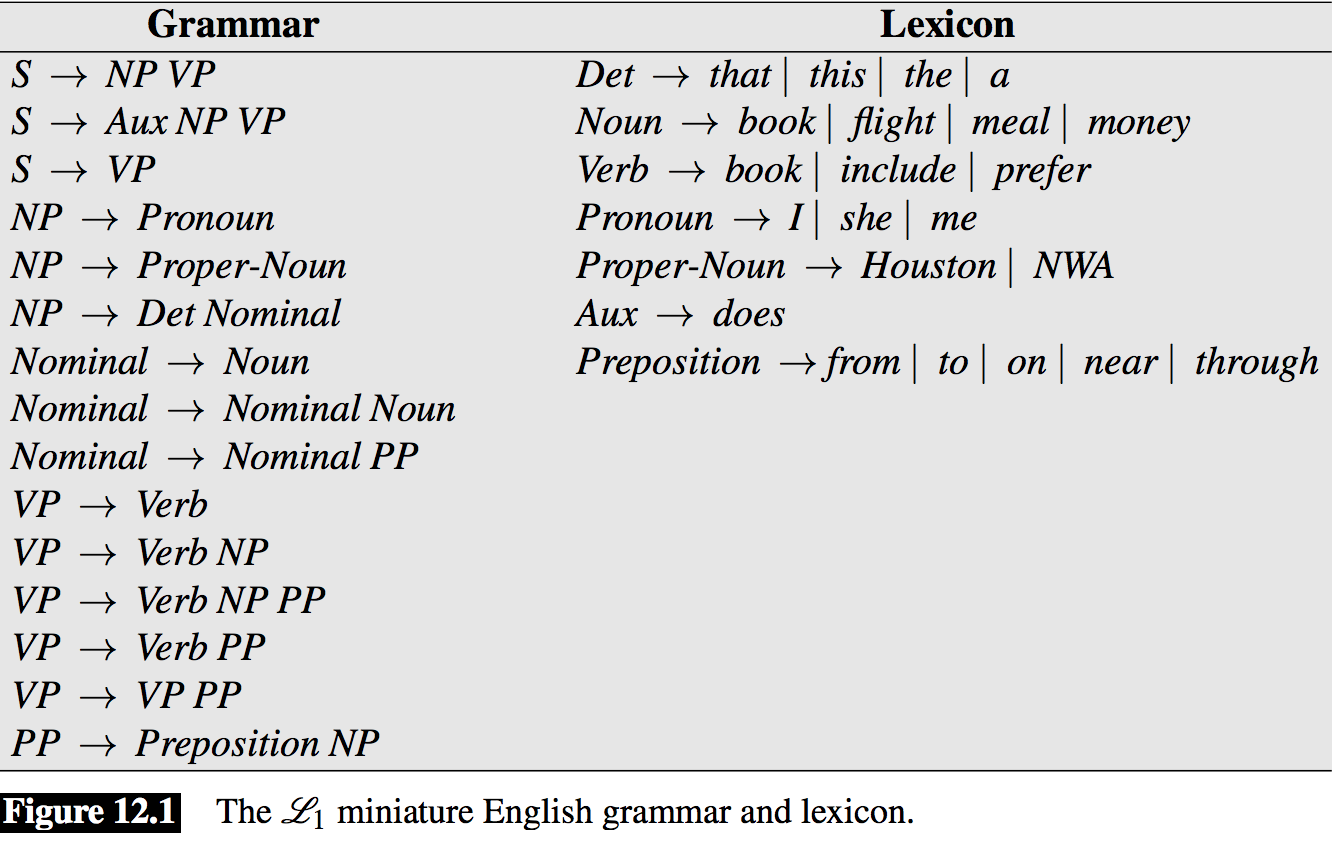
\includegraphics[width=\textwidth]{figures/grammar}
\end{frame}

\begin{frame}
\frametitle{Chomsky Normal Form}
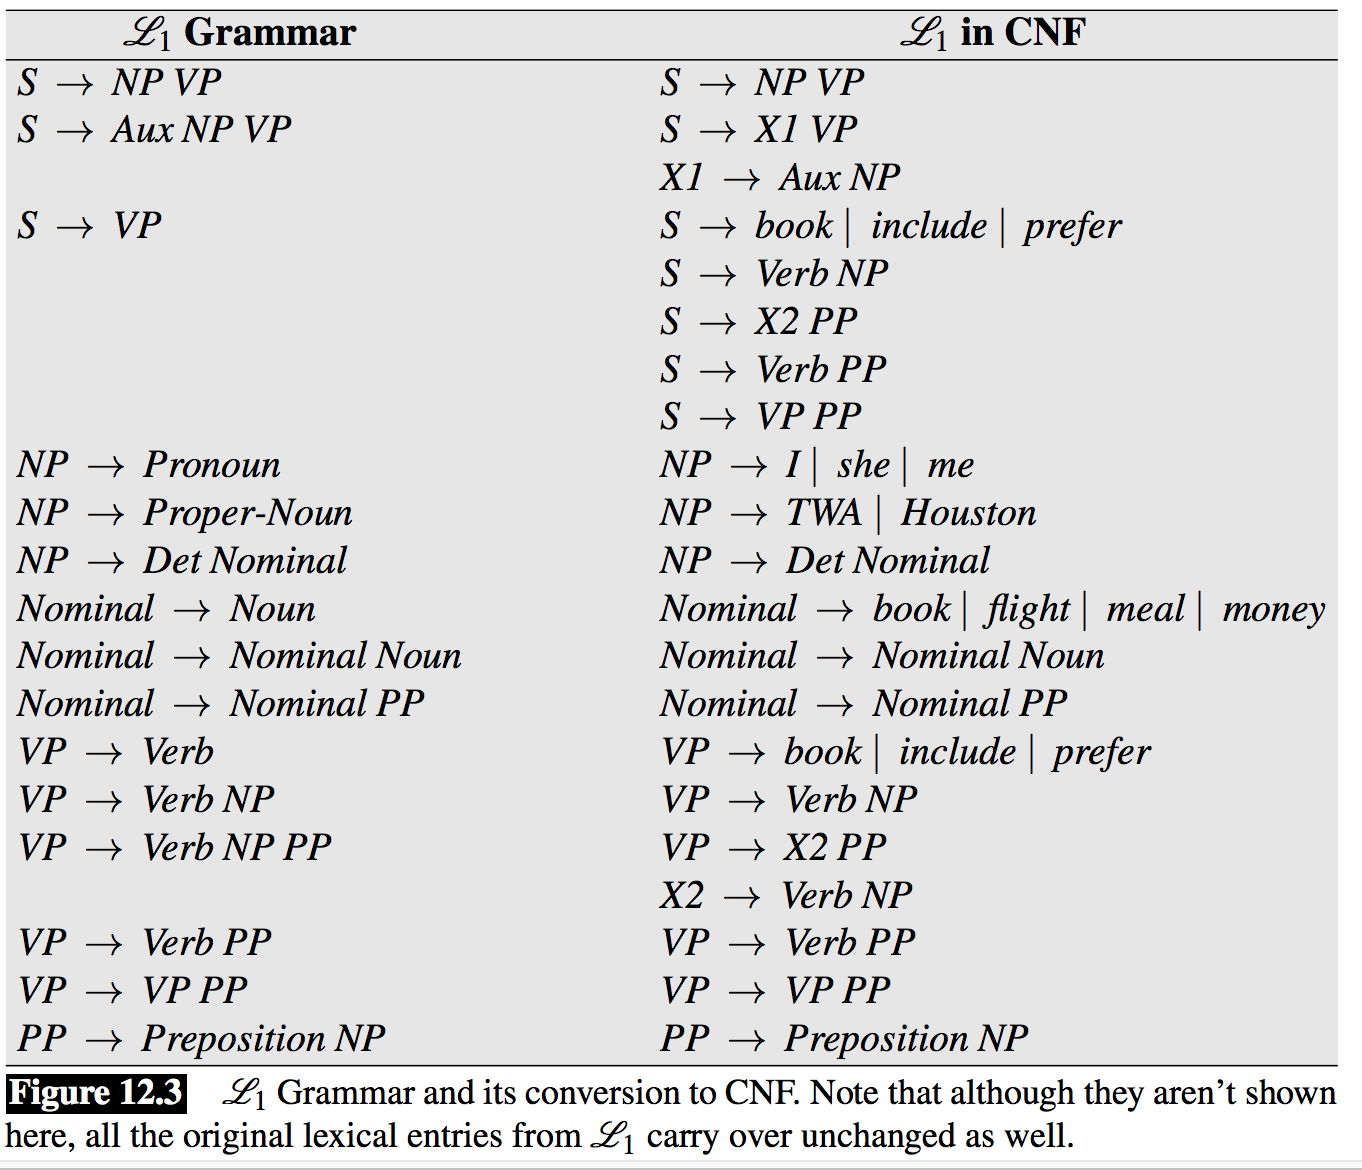
\includegraphics[width=\textwidth]{figures/CNF}
\end{frame}

\begin{frame}
\frametitle{CKY: Main idea}
\begin{itemize}
\item A 2-dimensional array (aka a table) can encode the structure of the tree
\item Each cell [i,j] contains all constituents that span positions {\it i} through {\it j} of the input string
\begin{itemize}
\item $_0Book_1that_2flight_3$
\end{itemize}
Cell [0,n] must have the Start symbol if we have a parse
\begin{itemize}
\item ...and can have more than one!
\end{itemize}
\end{itemize}
\end{frame}


\begin{frame}
\frametitle{CKY}
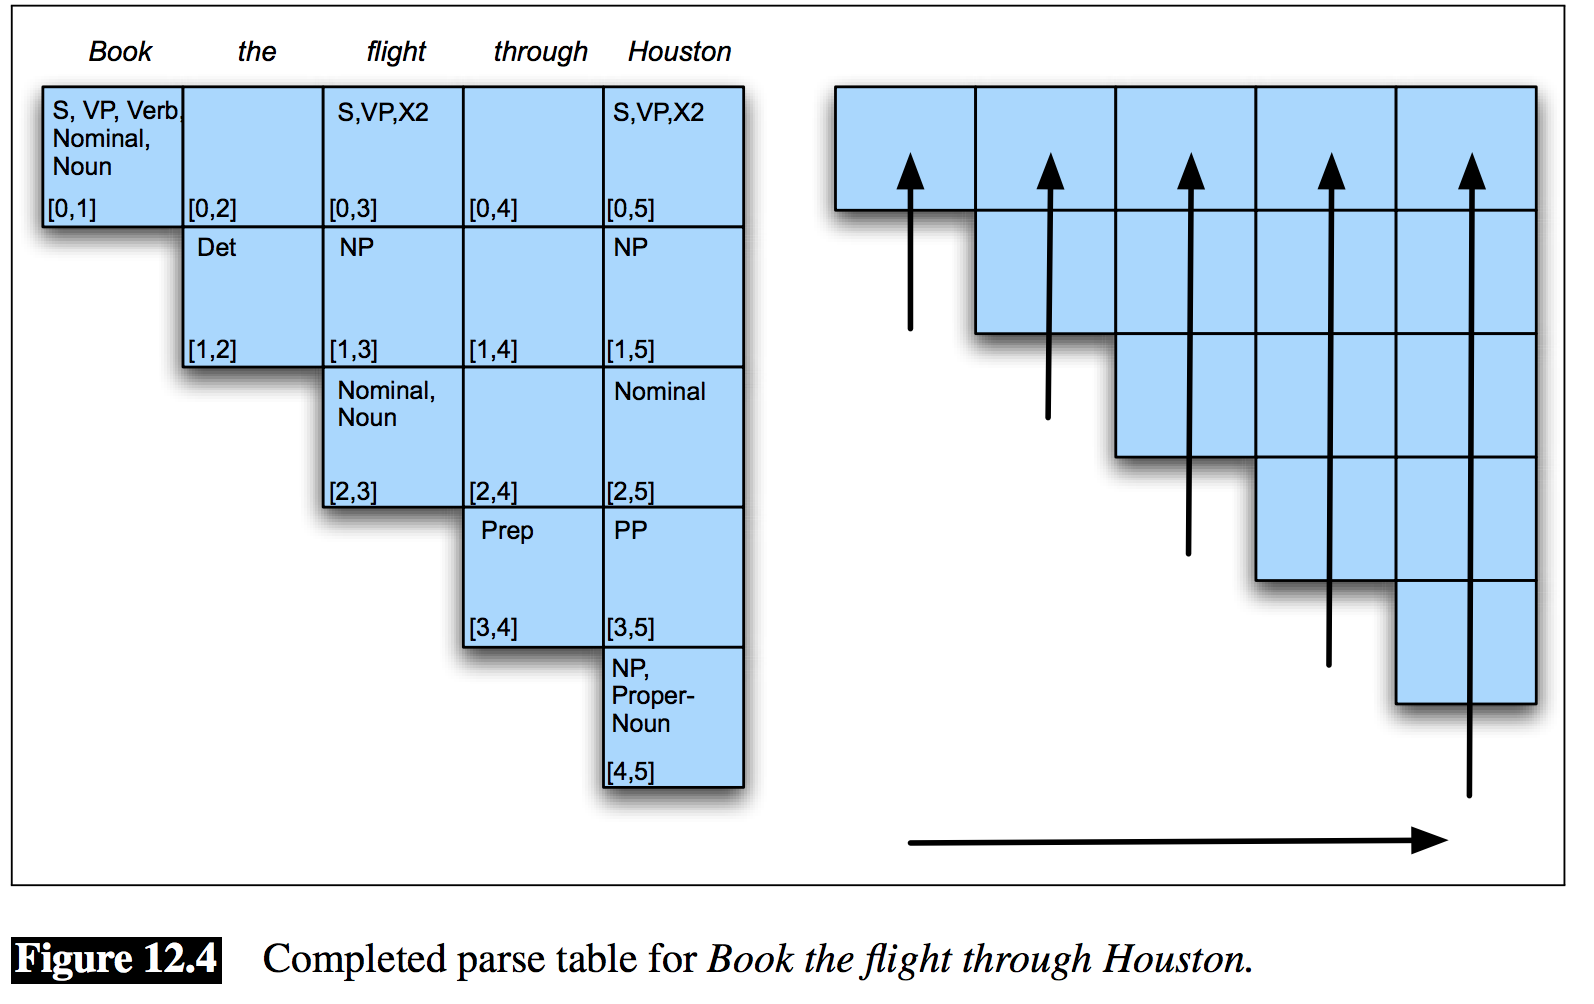
\includegraphics[width=\textwidth]{figures/cky1}
\end{frame}

\begin{frame}
\frametitle{CKY}
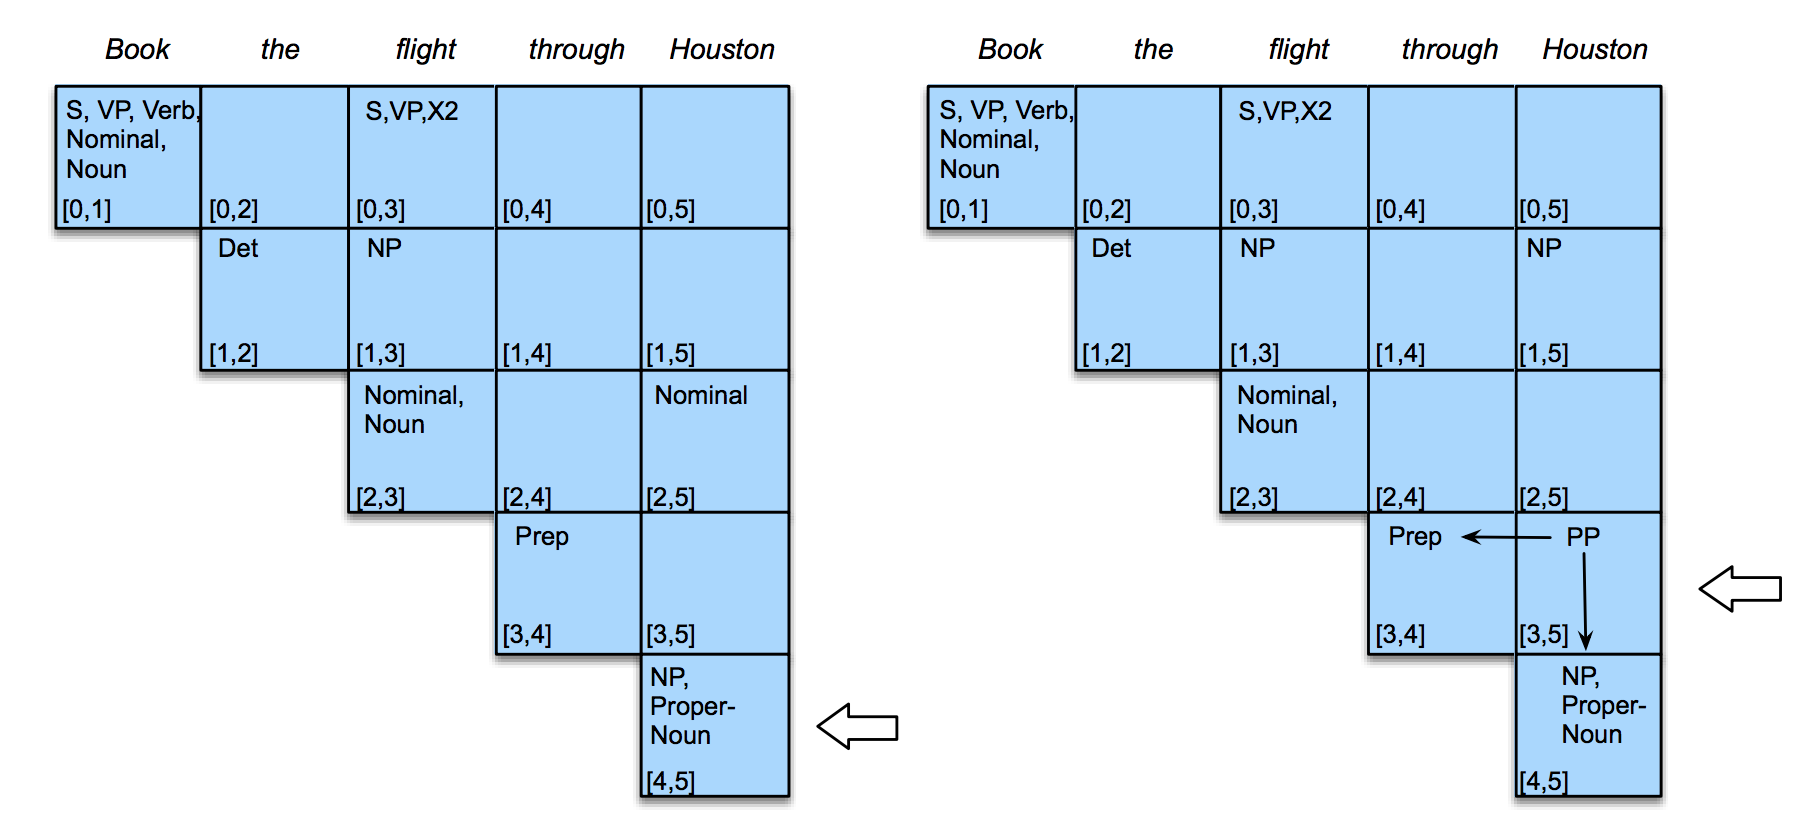
\includegraphics[width=\textwidth]{figures/cky2}
\end{frame}

\begin{frame}
\frametitle{CKY}
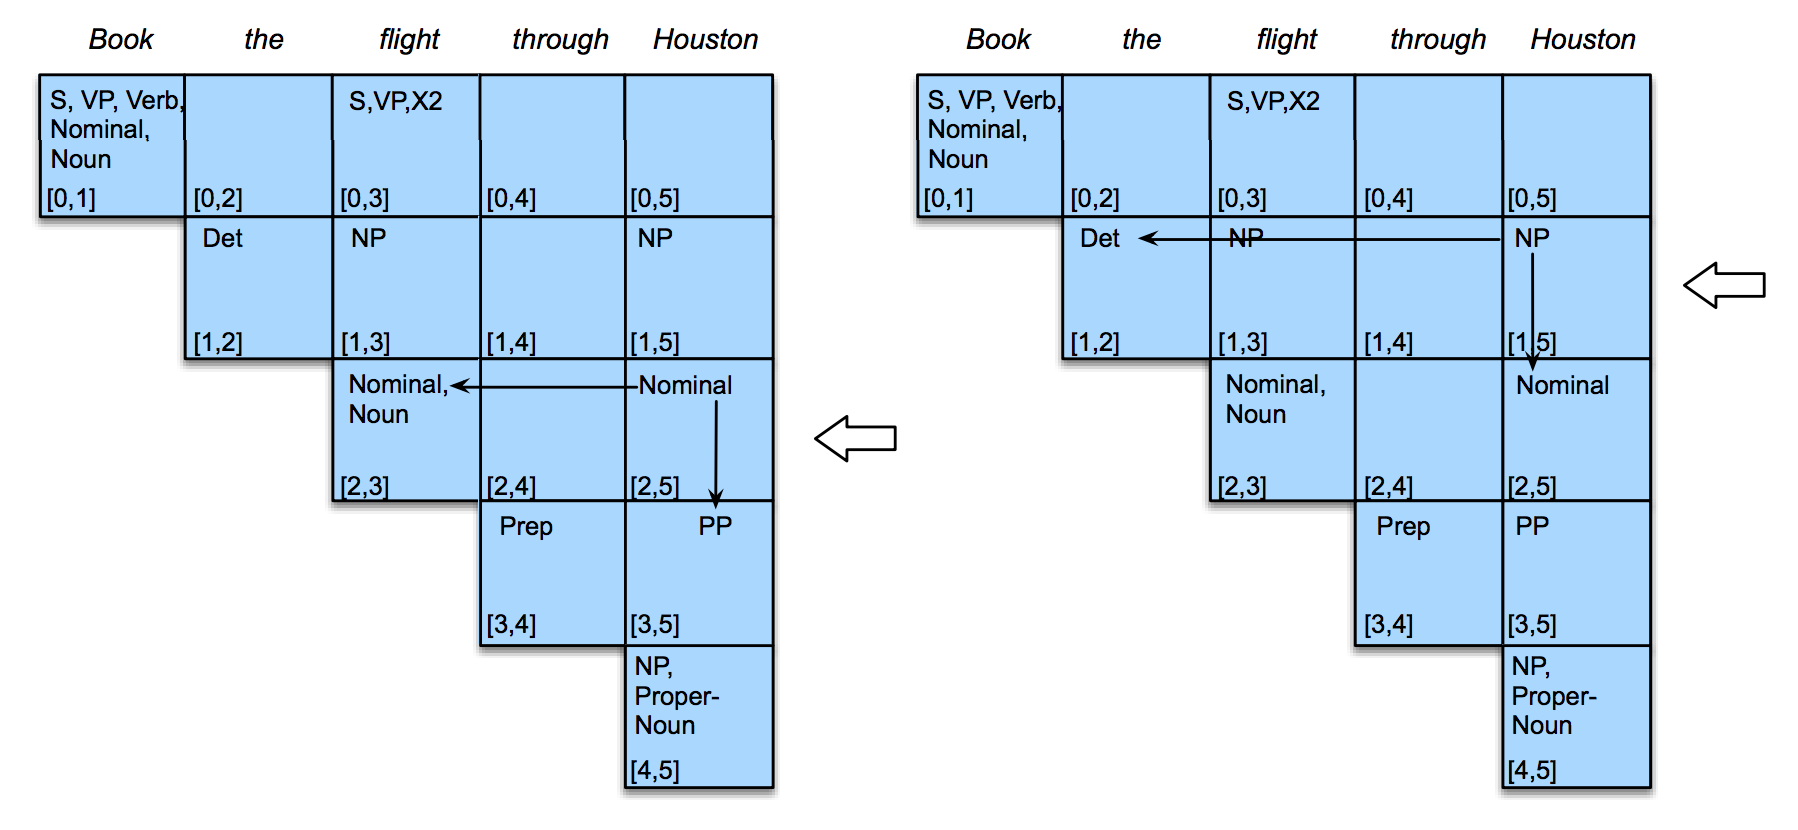
\includegraphics[width=\textwidth]{figures/cky3}
\end{frame}

\begin{frame}
\frametitle{CKY}
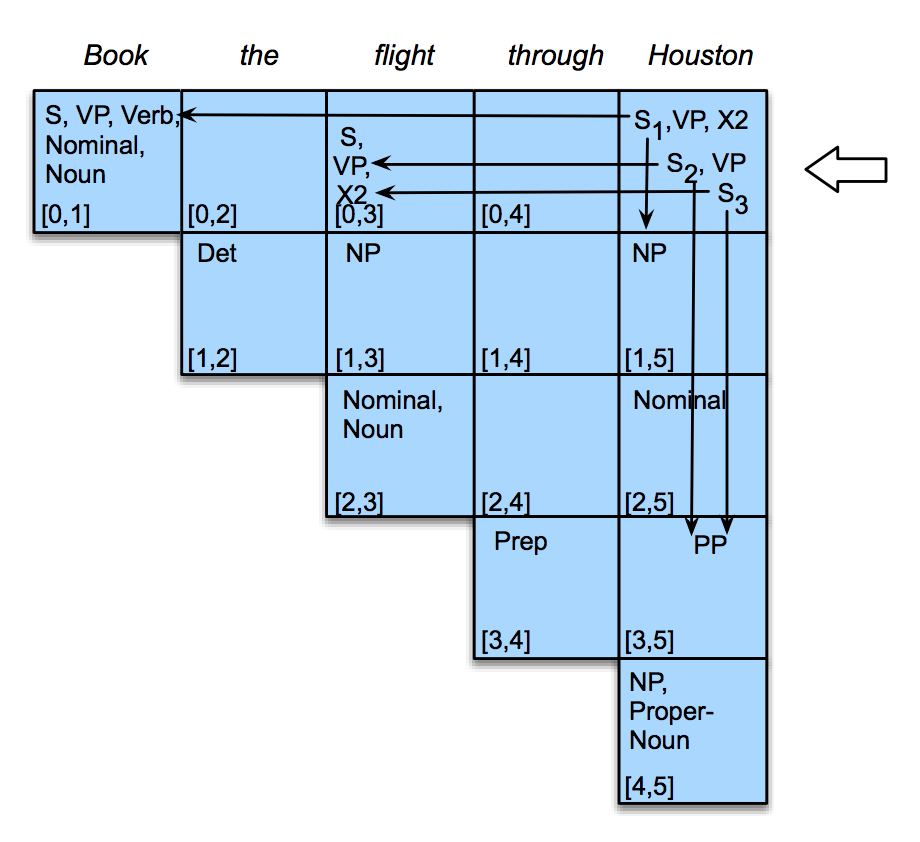
\includegraphics[width=\textwidth]{figures/cky4}
\end{frame}

\begin{frame}
\frametitle{Limitations of classical CKY}
\begin{itemize}
\item It is a recognizer
\item Turn a recognizer into a parser by storing all tree paths leading to S
\item ...but returning all possible trees is again exponential time!
\item Also, we modified the grammar!
\end{itemize}
\end{frame}


\begin{frame}
\frametitle{Limitations of classical CKY: Solutions}
\begin{itemize}
\item Probabilistic parsing
\item Train a probabilistic grammar and then return the most probable parse
\item Modify CKY to be able to recover original grammar
\item Employ e.g. partial parsing to get accommodate CFG directly (not in CNF)
\end{itemize}
\end{frame}

\end{document}

